\section{Auswertung}

    \subsection{Schallgeschwinidigkeit}

        \noindent Im ersten Versuchsteil wird die Schallgeschwindigkeit in Acryl berechnet. Dazu wurden mit dem Impuls-Echo-Verfahren 
        unterschiedliche Störstellen in einem Acrylblock vermessen. Die Daten dieser Messungen sind in Tabelle(\ref{tab:mess1}) zu finden.\\
        Werden diese geplotted und durch eine Ausgleichsgerade der Form $y = m \cdot x + b$ gefittet, ergibt sich Plot(\ref{img:py_sch}).

        \begin{figure}[ht]
            \centering
            \includegraphics[width=0.7\textwidth]{build/plots/Schallgeschwindigkeit.pdf}
            \caption{Die Messwerte geplottet und duch eine Ausgleichsgerade engenähert.}
            \label{img:py_sch}
        \end{figure}

        \noindent Die in diesem Plot dargestellte Ausgleichsgerade wird durch die Parameter: 
            \begin{align*}
                m &= \SI{1370.3(3)}{\metre\per\second}\\
                b &= \SI{-13.6(1)e-4}{\metre}       
            \end{align*}
        \noindent
        dargestellt.\\
        Die Steigung $m$ beschreibt hier bereits eine Geschwindigkeit, diese muss jedoch noch einmal verdoppelt werden, da bei dem 
        Impuls-Echo Verfahren die Strecke doppelt zurück gelegt wird. Somit berechnet dich die Schallgeschwindigkeit in Acryl zu : 
        \begin{equation*}
            c_{\text{Schall}} = 2 \cdot m = \SI{2741(7)}{\metre\per\second}
        \end{equation*}
        
    \subsection{Dämpfung}

        \noindent Um den Absorptionskoeffizient $\alpha$ der Schallamplitude aus der Formel:

        \begin{equation*}
            I(x) = I_0 \cdot \text{e}^{-\alpha x}
        \end{equation*}

        \noindent zu bestimmen werden die Schallamplituden gegen die Strecke geplottet.\\
        Die Amplituden sind auch in der 
        Tabelle(\ref{tab:mess1}) zu finden.\\ 
        Um systematische Fehler zu verhindern wurden für die Strecke nicht die per Schieblehre vermessenen 
        Werte benutzt sondern erneut aus $s = c_{\text{Scall}}\cdot t$ berechnet. Diese Messwerte wurden nun per scypy.curvefit \cite{scipy}
        an eine Funktion der Form

        \begin{equation*}
            I(x) = A * \text{e}^{B x}
            \label{eqn:fit}
        \end{equation*}

        \noindent gefittet. Dies ergibt dann insgesamt die Abbildung(\ref{img:py_daem}).

        \begin{figure}[ht]
            \centering
            \includegraphics[width=0.7\textwidth]{build/plots/Daempfung.pdf}
            \caption{Die Messwerte geplottet und duch eine Exponetialfunktion gefittet.}
            \label{img:py_daem}
        \end{figure}

        \noindent Hier berechnen sich die Parameter aus Gleichung(\ref{eqn:fit}) zu: 
        \begin{align*}
            A &= \SI{488(65)e-3}{\volt} \\
            B &= \SI{-23(3)}{\per\metre}    
        \end{align*}

        
        \noindent Somit wurde der Absorptionskoeffizient $\alpha$ zu:\\
        \begin{equation*}
            \alpha = -B = \SI{23(3)}{\per\metre}
        \end{equation*} 
        berechnet.

        \begin{table}[H]
            \centering
            \small
            \begin{tabular}{S [table-format=2.0] S [table-format=2.1] S [table-format=2.2]S [table-format=1.4]}
                \toprule
                {Messnummer } & {$s \mathbin{\scalebox{1.5} / }\si{\milli \metre} $} & {$t \mathbin{\scalebox{1.5} / }\si{\micro \second}$}& {$U \mathbin{\scalebox{1.5} / }\si{\volt}$}\\
                \midrule
                1   & 13.2    & 10.75   & 0.308 \\
                2   & 60.8    & 45.3    & 0.034 \\
                3   & 21.6    & 16.8    & 0.195 \\
                4   & 53.3    & 39.8    & 0.043 \\
                5   & 30.3    & 23.2    & 0.126 \\
                6   & 45.4    & 34.3    & 0.032 \\
                7   & 38.8    & 29.4    & 0.074 \\
                8   & 38.0    & 28.9    & 0.069 \\
                9   & 46.7    & 35.2    & 0.057 \\
                10  & 30.0    & 22.9    & 0.110 \\
                11  & 54.7    & 41.0    & 0.042 \\
                12  & 21.9    & 17.1    & 0.135 \\
                13  & 62.8    & 46.8    & 0.026 \\
                14  & 13.8    & 11.2    & 0.222 \\
                16  &  6.8    &  5.4    & 0.300 \\ 
                17  & 15.5    & 12.4    & 0.365 \\
                18  & 54.6    & 40.8    & 0.039 \\
                19  & 59.0    & 44.0    & 0.0022\\
                20  & 19.5    & 15.1    & 0.124 \\
                21  & 60.7    & 45.4    & 0.0024\\
                22  & 17.8    & 13.9    & 0.135 \\
                23  & 80.0    & 59.1    & 0.029 \\  
                \bottomrule
            \end{tabular}
        \caption{Messdaten der Ultraschalluntersuchung eines Acrylblocks mit Störstellen. Die einzelnen Störstellen wurden von oben 
        und von unten vermessen. Hier beschreibt somit immer eine aufeinander folgende ungerade und dann gerade Messnummer eine Störstelle,
        jediglich Messnummer 15 konnte nicht aufgenommen werden da die Störstelle von einer größeren Störstelle verdeckt wurde. Messnummer 23 
        ist der am Tisch reflektierter Impuls.}
        \label{tab:mess1}
        \end{table}


    \subsection{Augenmodell}

        \noindent Aus dem Bild(\ref{img:Auge_dat}) lassen sich 3 Peaks ablesen, diese sind bei $t_1 = \SI{17.4}{\micro \second}$, 
        $t_2 = \SI{18.2}{\micro \second}$ und bei $t_3 = \SI{23.1}{\micro \second}$. Der erste Peak entsteht hier durch die Reflektion an der Iris, 
        der zweite an der Linse und der dritte hinten an der Retina. Über diese Zeiten lassen sich nun mittels der spezifischen 
        Schallgeschwinidigkeiten in der Linse $c_{\text{L}} = \SI{2500}{\meter\per\second}$ und in der Glaskörperflüssigkeit 
        $c_{\text{GK}} = \SI{1410}{\meter\per\second}$, die Abmaße des Augenmodells bestimmen \cite{US1}. 

        \begin{align*}
             s_{\text{I}} & = \frac{1}{2} t_1 c_{\text{GK}}                      &= \SI{12.267}{\milli\metre}   \\
             s_{\text{L}} & = s_{\text{I}} + \frac{1}{2} (t_2-t_1) c_{\text{L}}  &= \SI{13.267}{\milli\metre}  \\
             s_{\text{R}} & = s_{\text{L}} + \frac{1}{2} (t_3-t_2) c_{\text{GK}} &= \SI{22.362}{\milli\metre} 
        \end{align*}

        \noindent Hier ist $s_{\text{I}}$ der Abstand bis zur Iris, $s_{\text{L}}$ der Abstand bis zur Linse und $s_{\text{R}}$ der Abstand 
        bis zur Retina.

        \begin{figure}[h]
            \centering
            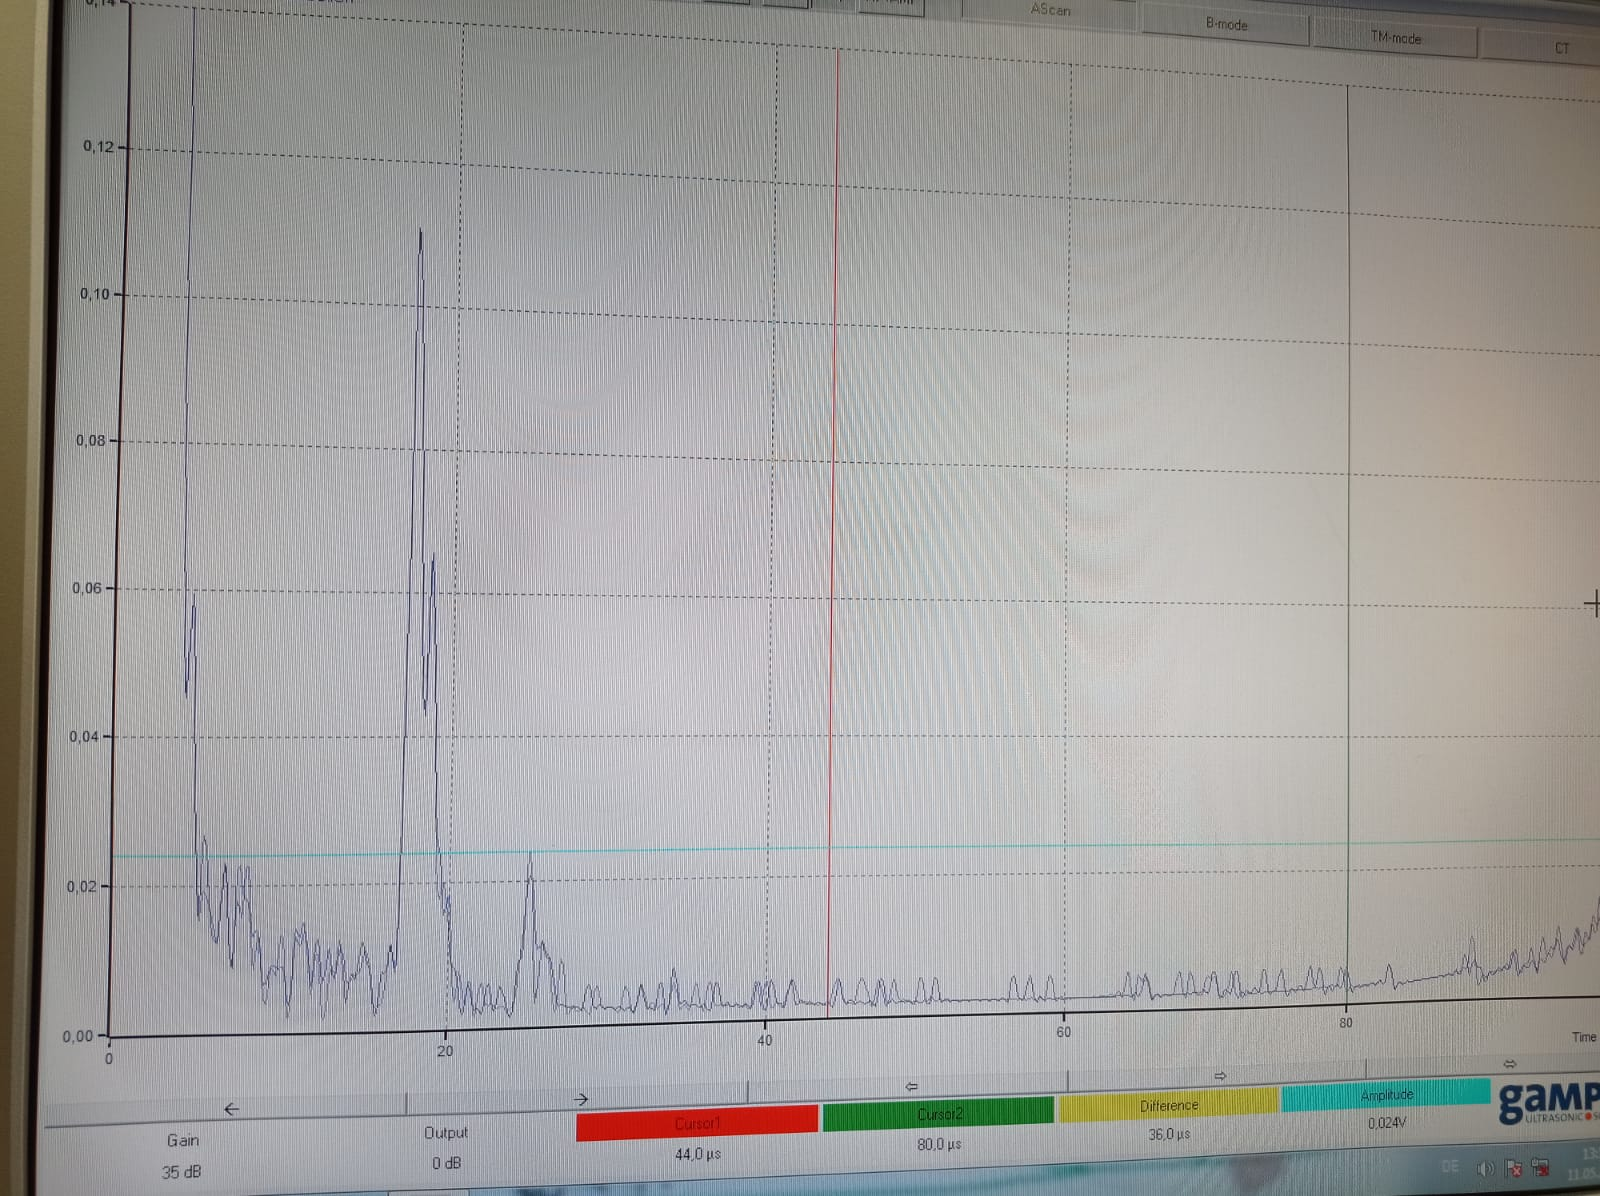
\includegraphics[width=0.7\textwidth]{latex/images/Auge_dat.jpeg}
            \caption{Aufnahme vom Echoskop beim vermessen des Augenmodells.}
            \label{img:Auge_dat}
        \end{figure}